\documentclass[tikz,border=2pt]{standalone}
\usepackage{amsmath}
\usepackage{pgfplots}
\pgfplotsset{compat=1.18}
\usetikzlibrary{arrows.meta}
\begin{document}
% Closed two-station cycle, E[S_1]=2, E[S_2]=1, n=3. Wide bars: time-average p_3(k)=P(L_1=k)=(1,2,4,8)/15.
% Narrow bars: distribution of the number at station 1 seen by an arriving job, (1,2,4,0)/7 = p_2(k),
% the time-average law of the network with n-1=2 jobs (arrival theorem).
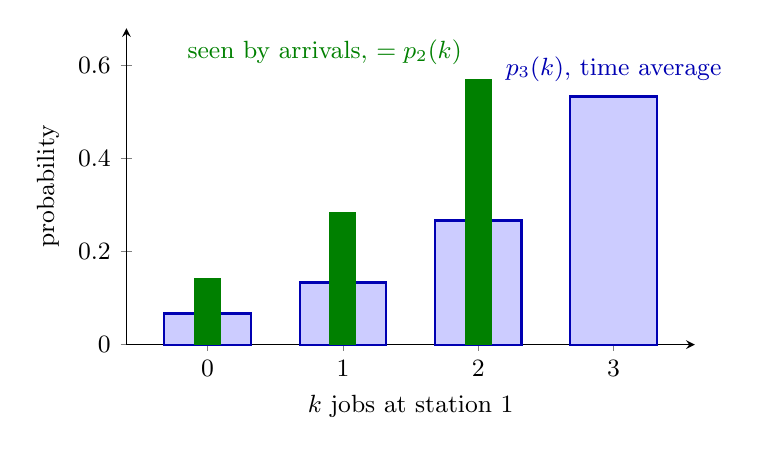
\begin{tikzpicture}[font=\small, >={Latex[length=2mm]}]
\begin{axis}[width=8.8cm, height=5.6cm, axis lines=left,
  xmin=-0.6, xmax=3.6, ymin=0, ymax=0.68,
  xtick={0,1,2,3}, ytick={0,0.2,0.4,0.6},
  yticklabel style={/pgf/number format/fixed},
  xlabel={$k$ jobs at station 1}, ylabel={probability},
  clip=false]
  \foreach \k/\v in {0/0.0667,1/0.1333,2/0.2667,3/0.5333} {
    \edef\temp{\noexpand\draw[thick, blue!70!black, fill=blue!20] (axis cs:\k-0.32,0) rectangle (axis cs:\k+0.32,\v);}
    \temp
  }
  \foreach \k/\v in {0/0.1429,1/0.2857,2/0.5714} {
    \edef\temp{\noexpand\fill[green!50!black] (axis cs:\k-0.1,0) rectangle (axis cs:\k+0.1,\v);}
    \temp
  }
  \node[blue!70!black, anchor=south] at (axis cs:3,0.545) {$p_3(k)$, time average};
  \node[green!50!black, anchor=south east] at (axis cs:1.95,0.58) {seen by arrivals, $=p_2(k)$};
\end{axis}
\end{tikzpicture}
\end{document}
